\chapter{LITERATURE REVIEW}

\section{Existing Works}
Brain-computer interfaces, are systems that let a person communicate with a computer using signals from the brain. These systems read brain activity and turn it into signals that a computer or device can understand, without needing things like a keyboard or mouse. BCIs can be grouped based on how they record brain signals. The main types include:\begin{itemize}
	\item \gls{eeg}
	\item Functional magnetic resonance imaging (fMRI)
	\item Near infrared spectroscopy (NIRS)
	\item Magnetoencephalography (MEG)
	\item Electrocorticography (ECoG)

\end{itemize}

EEG is a non-invasive method that records the electrical activity of the brain using electrodes placed outside the head in the scalp. ECoG is different because it is invasive and places electrodes directly on the surface of the brain to measure electrical activity. ECoG can give better accuracy than EEG, but because it is invasive, but this requires extensive surgery and includes risk to the user. MEG, fMRI, and NIRS are also non-invasive methods, but these require big industrial equipment. MEG measures the magnetic fields created by brain activity. fMRI uses strong electromagnetic fields and in BCI applications usually measures blood oxygen level dependent (BOLD) changes linked to neural activity. NIRS uses infrared light that can pass a short distance through the skull and measures the reflected light. More detailed descriptions of all these methods can be found in \cite{nicolas2012bci}.

\section{EEG Based BCI}
Focusing again on EEG based BCIs, there are several types of brain signals that can be used to send commands to a computer or other device. Some common examples include sensorimotor rhythms (SMRs), visually evoked potentials (VEPs), and slow cortical potentials (SCPs) . Each of these signals works in a different way and is useful for different kinds of BCI systems. In many practical and research based applications, VEPs and SMRs are among the most widely used because they can provide clear control signals and are well studied in the field. For this reason, these two EEG signal types are especially important and will be described in the following sections.

Visual evoked potentials, often called VEPs, are brain responses that appear when a person sees a visual stimulus. These signals can be observed from the occipital region, which is located at the back of the head and is strongly related to visual processing. When the visual stimulus flashes repeatedly at a constant frequency, the brain produces a repeating response of the identical frequency. This type of response is known as a steady state visually evoked potential, or SSVEP. In this type of system the user selects commands by looking a particular flickering pattern.

Even though VEP based systems have been extensively studied for BCI applications, this is not the emphasis of the current study. The current study emphasizes a different approach to VEP. An instance of SSVEP based application is an interface that resembles a keyboard where each character corresponds to a light source which flickers at a distinct frequency. It is possible to know what character the user is focused on by analyzing the frequency domain components of the EEG signal of the user. This allows us to determine the selected character based on the dominant frequency component of the occipital EEG signal  \cite{hwang2012ssvep}.


\section{Brain Waves and Their Relevance to the Proposed BCI System}
Electroencephalography (EEG) is an electrical activity of the brain registered in the form of waves, which belong to certain frequency ranges and represent particular mental or physiological conditions of a person. Delta waves (0.1 – 3 Hz) are the slowest waves that appear during deep dreamless sleep or when a person is unconscious. Theta waves (4 – 7 Hz) are associated with creative work, imagination, memory recollection and light sleeping or dreaming. They usually appear when a person's mind is relaxed and inwardly focused. Alpha waves (8 – 12 Hz) appear when a person is awake and relaxed. Such waves increase when a person's eyes are closed and decrease when he/she concentrates on something. Low beta waves (12 – 15 Hz) indicate relaxed but focused mental activities while mid range beta waves (16 – 20 Hz) reflect active thinking, problem solving and high awareness of the environment. High beta waves (21 – 30 Hz) appear when a person is highly alert, stressed or agitated. Gamma waves (30 – 100 Hz) are associated with higher mental processes like information processing, learning and memory integration. In the case of the suggested brain-computer interface (BCI) system, beta waves are to be used as control waves because they are clearly distinguished by their changes between relaxed and focused states allowing a simple and reliable interaction through the EEG-based interface. Although the other waves are not used for controlling the device directly, knowledge about all waves is crucial for proper filtering of noise and detecting beta waves activity.

\newpage
\begin{table}
	\centering
	\caption{\centering EEG frequency bands and associated mental states-Image Source: M.G.N.Garcia et al \cite{malmivuo1995bioelectromagnetism})}
	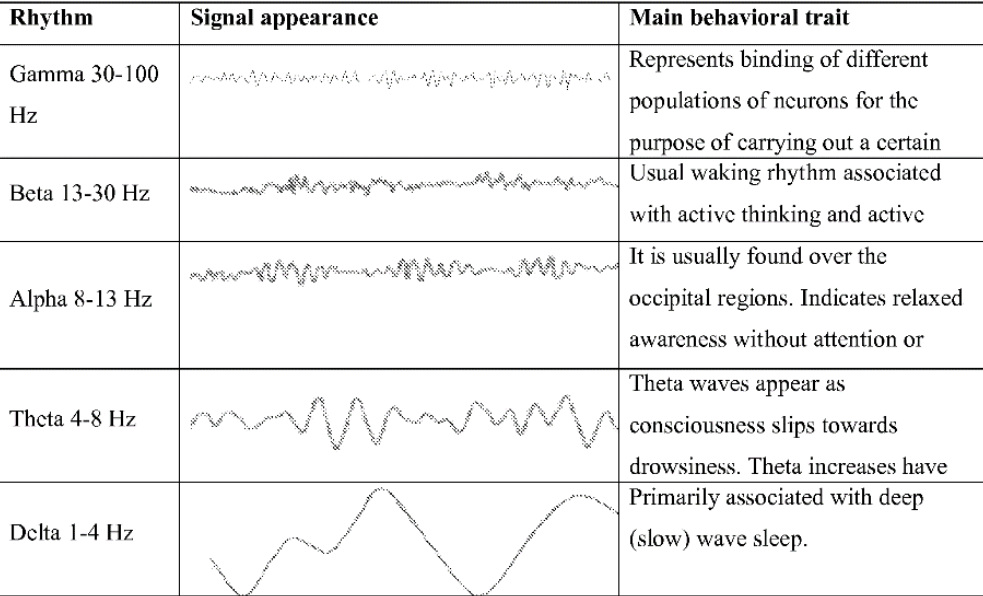
\includegraphics[width = 14cm]{src/images/figures/eeg_frequency_bands.png}
\end{table}

\vspace{10pt}
\section{Electroencephalography}
An EEG, or electroencephalogram, is a machine that can measure the tiny electrical signals our brain produces. We put small electrodes on the scalp to record these signals. People use EEG for many things like checking if someone is awake, seeing how they react to things around them, or finding sleep and brain problems. Lately, scientists started using EEG signals to control computers, which is called a BCI system \cite{vidal1973bci}.

The signals an EEG picks up depend on where the electrodes are placed and what the brain is doing at that moment. This is because different parts of the brain do different jobs. The most common way to put the electrodes on the head is called the 10-20 system \cite{malmivuo1995bioelectromagnetism}.

\begin{figure}
	\centering
	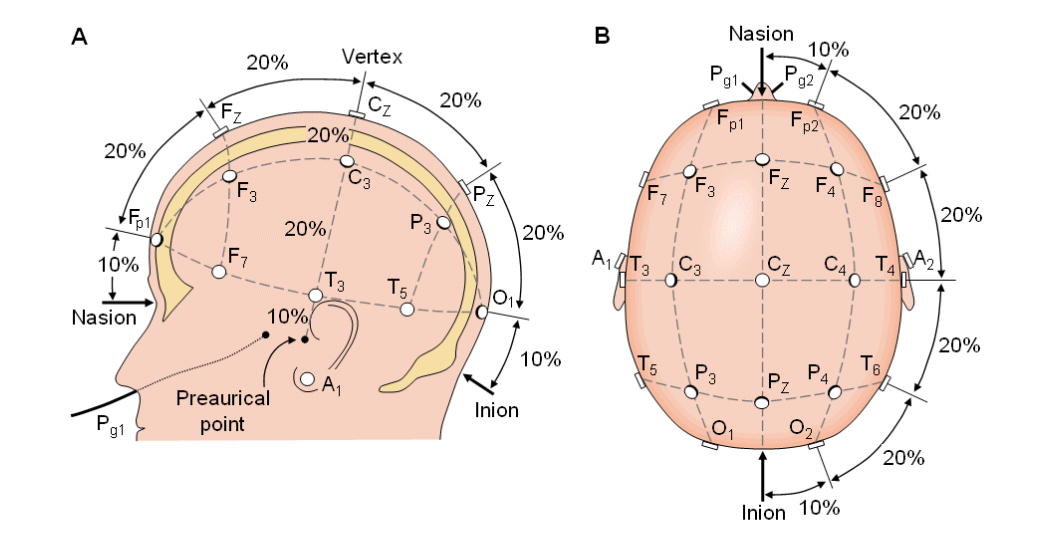
\includegraphics[width = 14cm]{src/images/figures/electrode_placement.png}
	\caption{\centering An example of the stimulation frequency arrangements (Image from H. Han Jeong \cite{hwang2012ssvep})}
\end{figure}
